\documentclass[12pt, twoside]{article}
\usepackage[francais]{babel}
\usepackage[T1]{fontenc}
\usepackage[latin1]{inputenc}
\usepackage[left=7mm, right=1cm, top=1cm, bottom=7mm]{geometry}
\usepackage{float}
\usepackage{graphicx}
\usepackage{array}
\usepackage{multirow}
\usepackage{amsmath,amssymb,mathrsfs} 
\usepackage{soul}
\usepackage{textcomp}
\usepackage{eurosym}
 \usepackage{variations}
\usepackage{tabvar}

\begin{document}


\textbf{Exercice 1}

\enskip

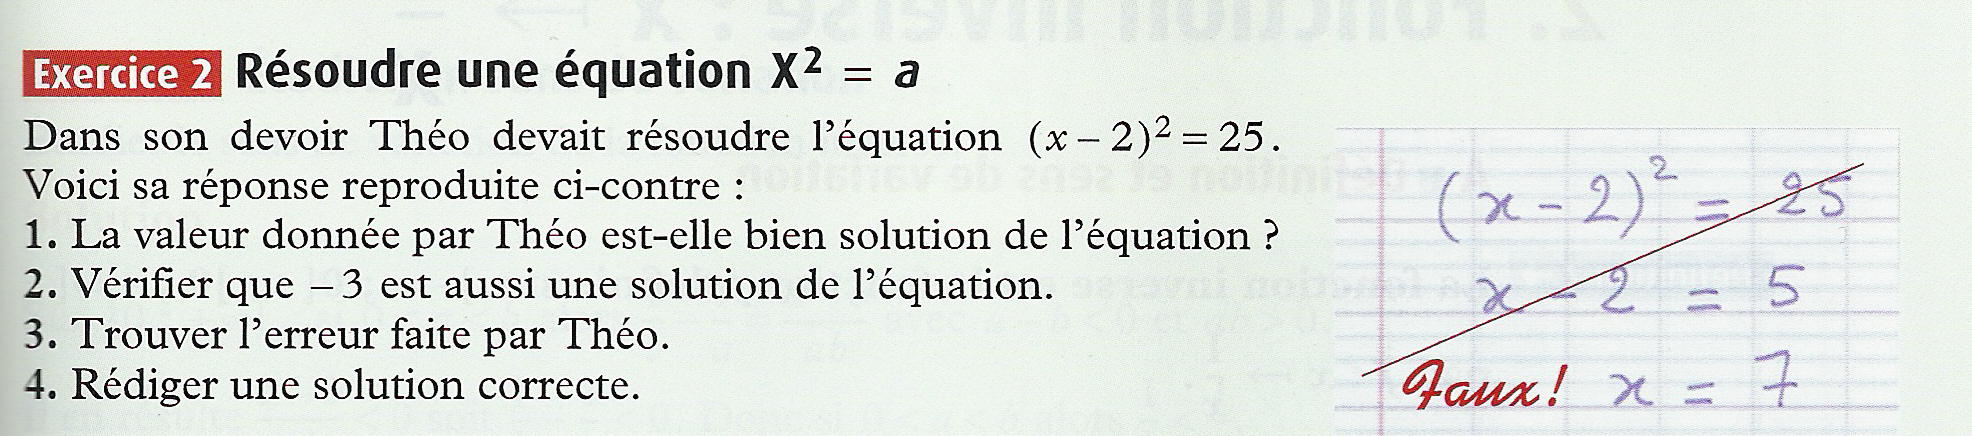
\includegraphics[width=13cm]{images/theo.png}



\medskip

\textbf{Exercice 1}

\enskip

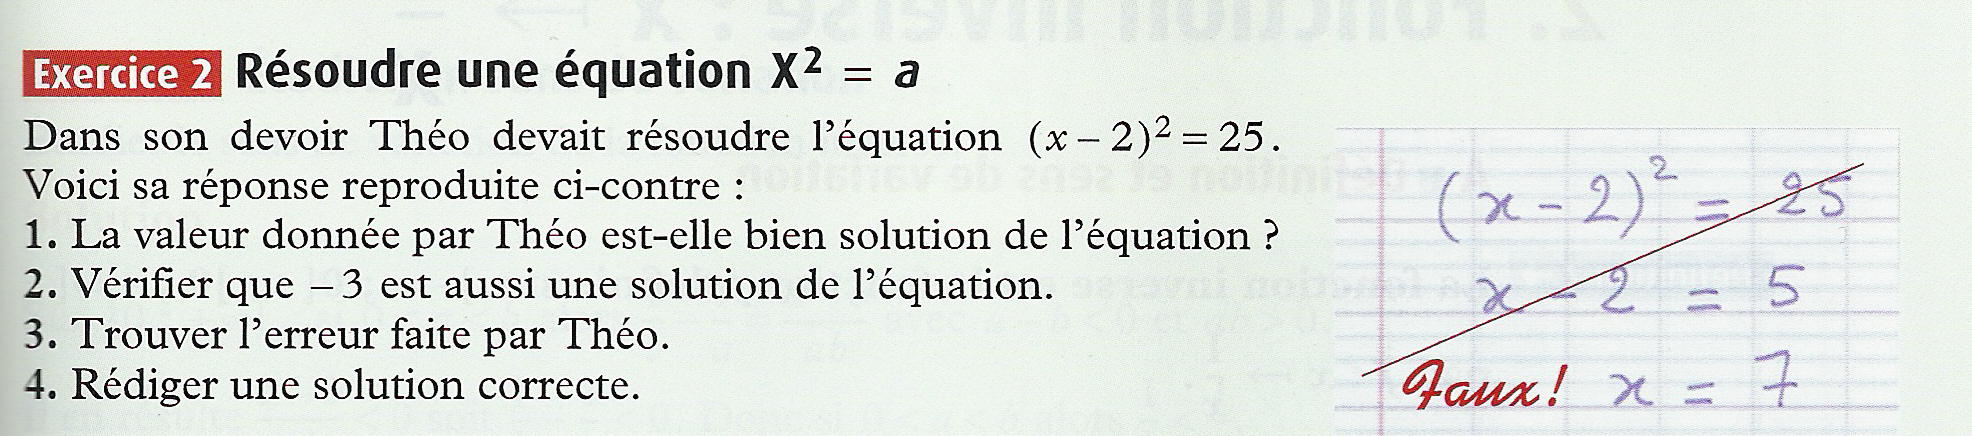
\includegraphics[width=13cm]{images/theo.png}



\medskip

\begin{tabular}{cc}
\begin{minipage}{9cm}
\textbf{Exercice 3}

\enskip

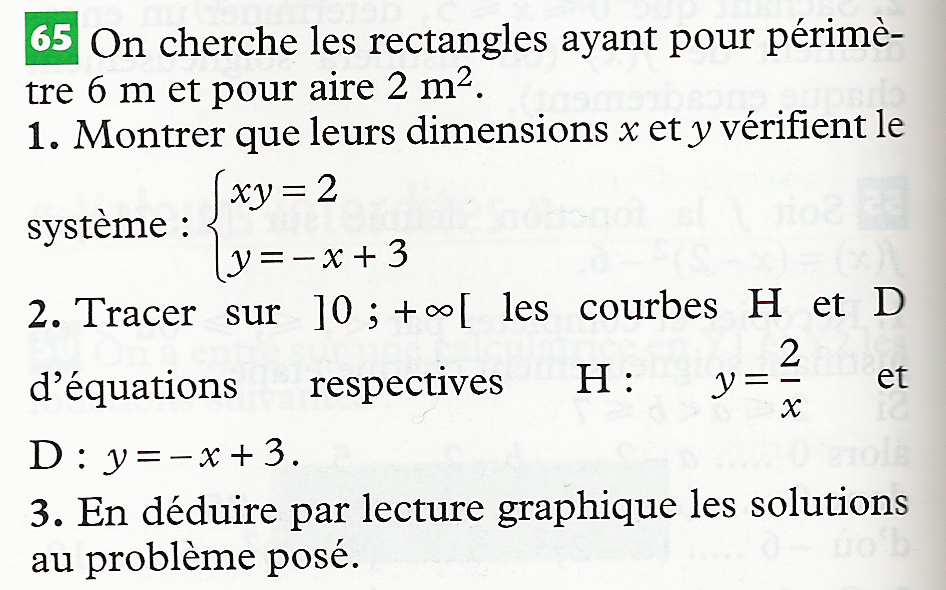
\includegraphics[width=7cm]{images/ineq2.png}
\end{minipage}
&
\begin{minipage}{9cm}
\textbf{Exercice 3}

\enskip

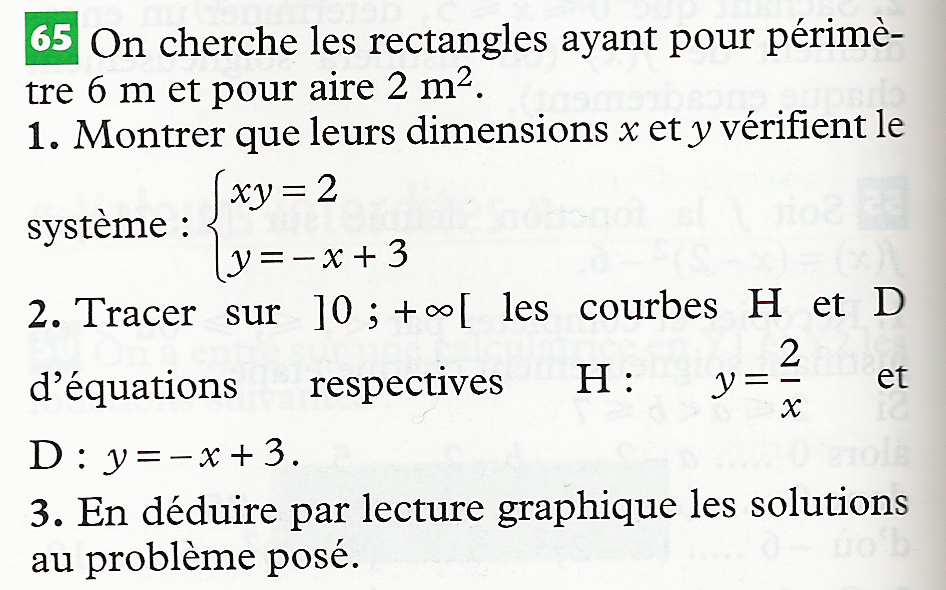
\includegraphics[width=7cm]{images/ineq2.png}
\end{minipage}
\end{tabular}

\medskip

\begin{tabular}{cc}
\begin{minipage}{9cm}
\textbf{Exercice 2}

\enskip

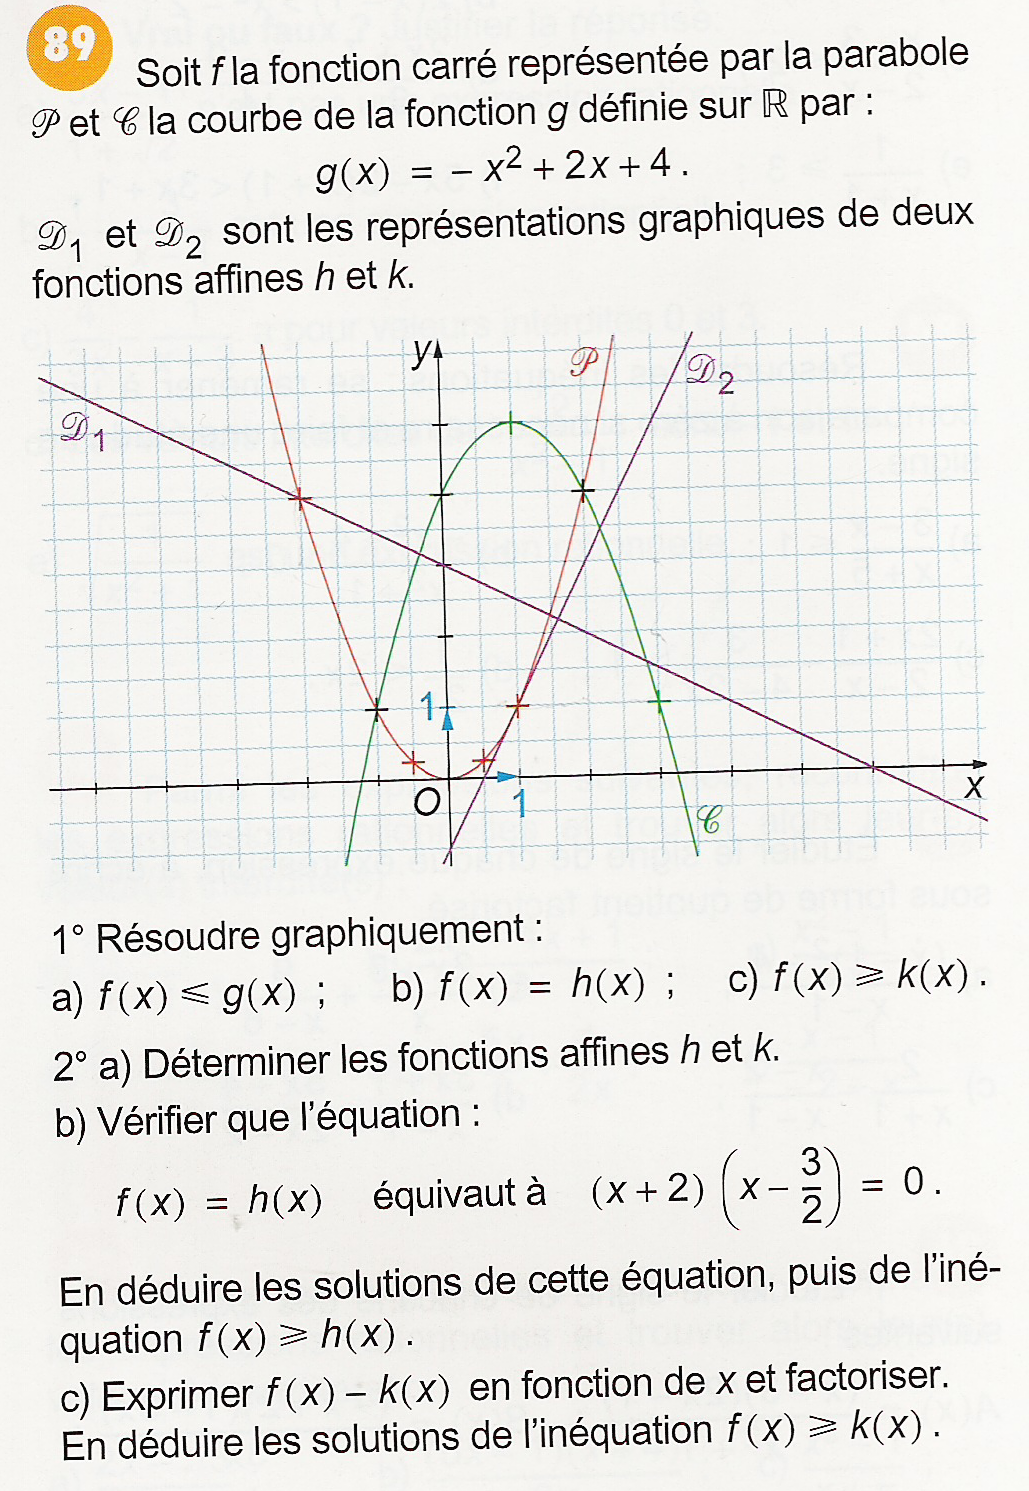
\includegraphics[width=8cm]{images/ineq1.png}
\end{minipage}
&
\begin{minipage}{9cm}
\textbf{Exercice 2}

\enskip

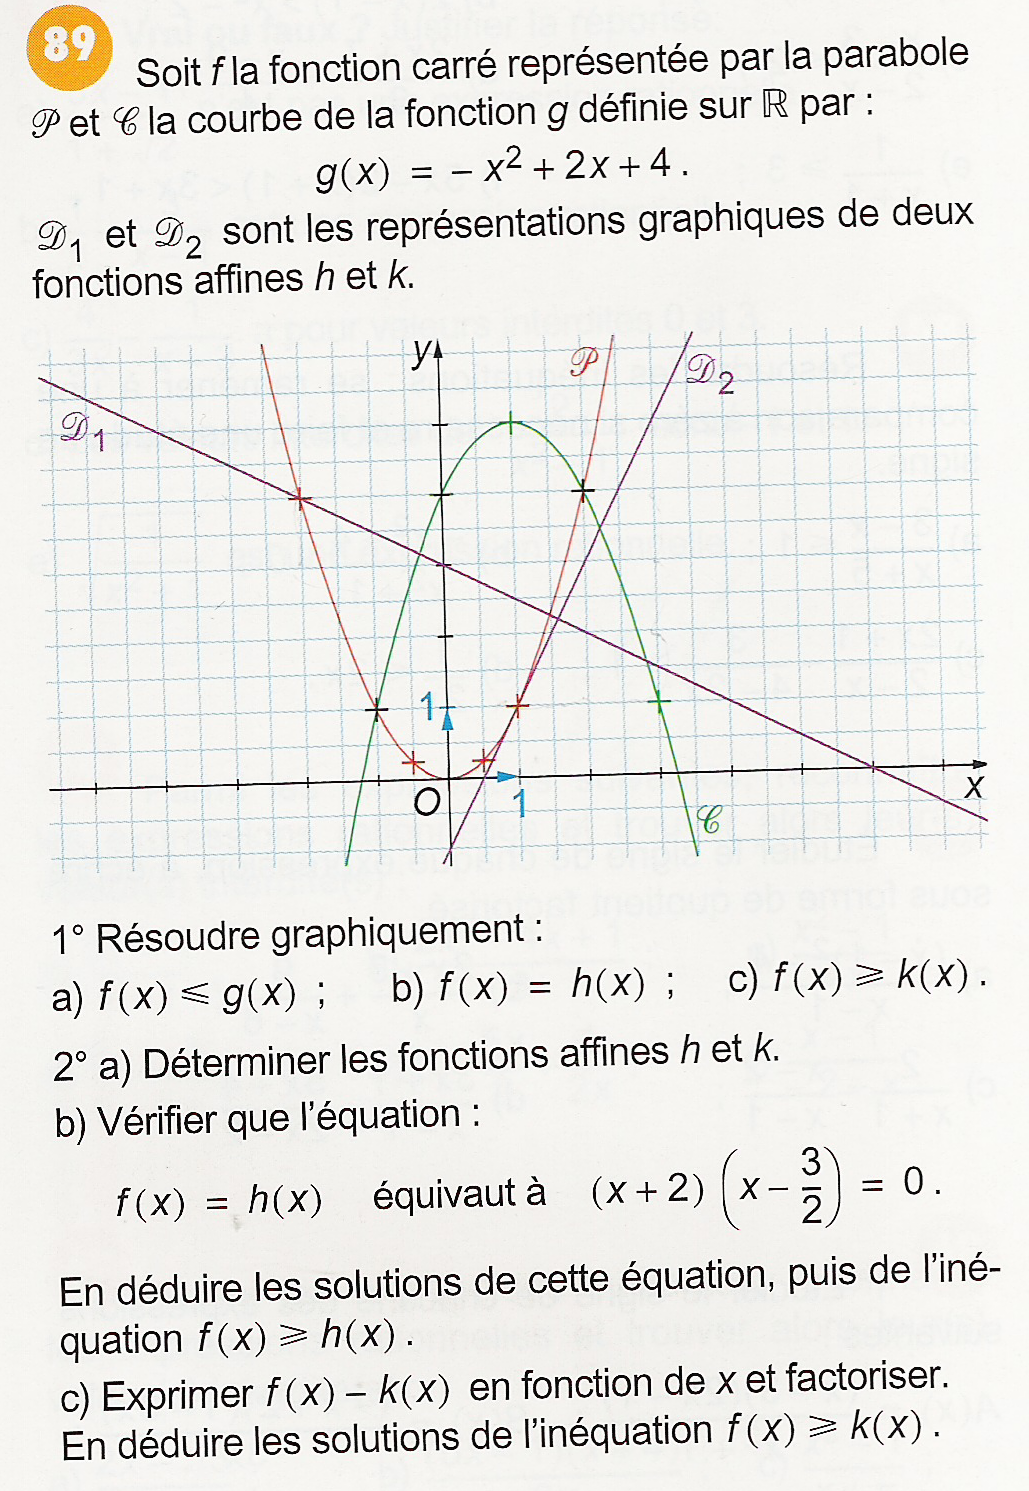
\includegraphics[width=8cm]{images/ineq1.png}
\end{minipage}
\end{tabular}

\pagebreak



\textbf{Exercice 4}

\bigskip

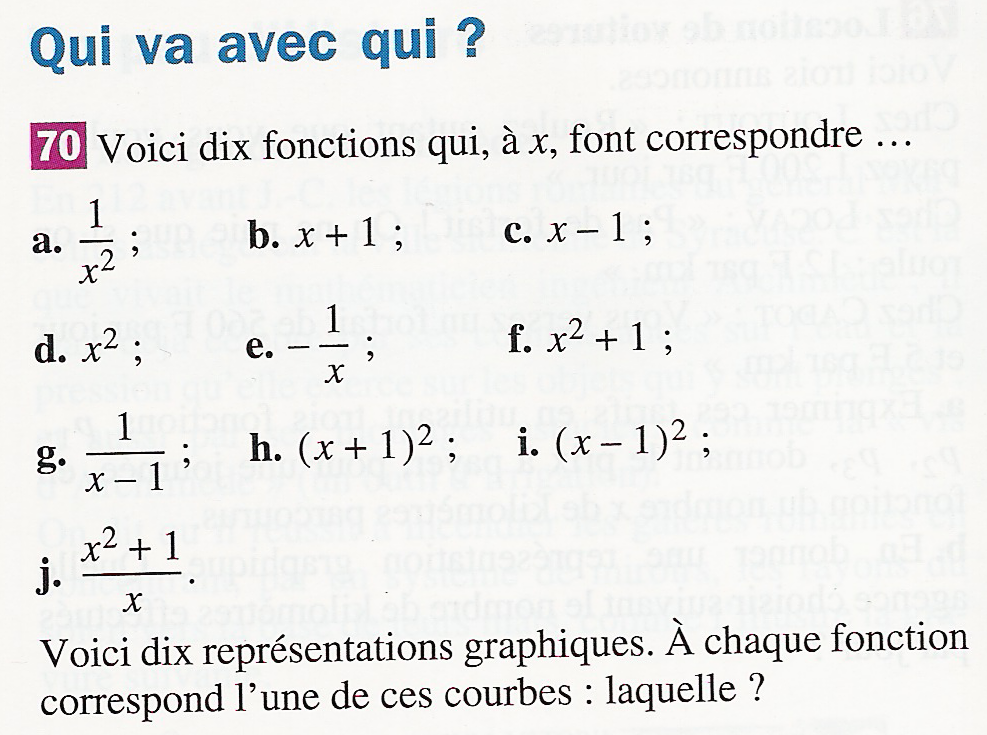
\includegraphics[width=8cm]{images/synthese.png} \qquad \quad \quad
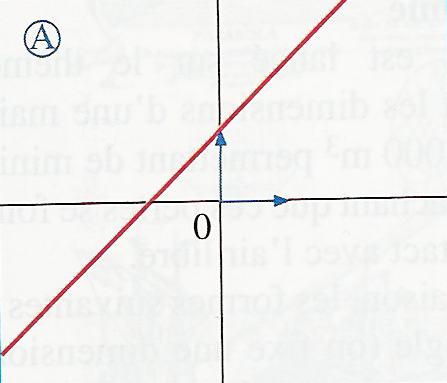
\includegraphics[width=5cm]{images/A.png} 

\bigskip

\bigskip

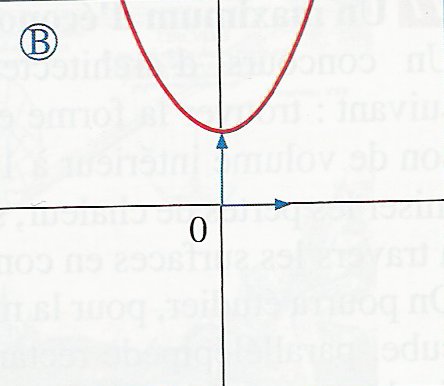
\includegraphics[width=5cm]{images/B.png} \qquad \quad \quad
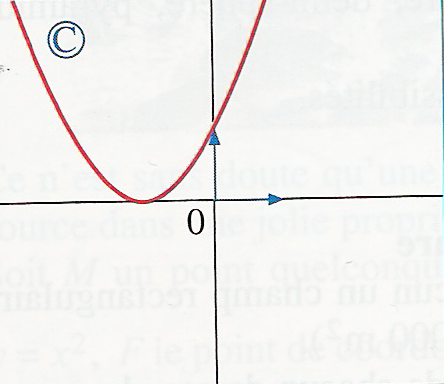
\includegraphics[width=5cm]{images/C.png} \qquad \quad \quad
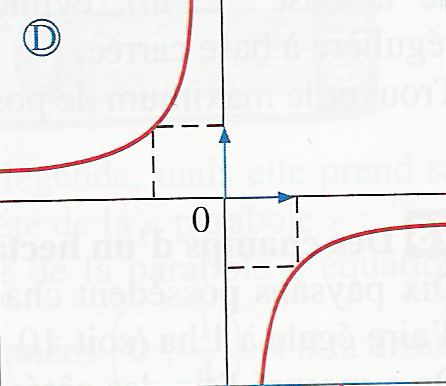
\includegraphics[width=5cm]{images/D.png} 

\bigskip

\bigskip

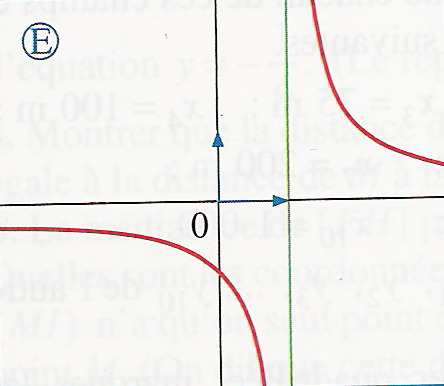
\includegraphics[width=5cm]{images/E.png} \qquad \quad \quad
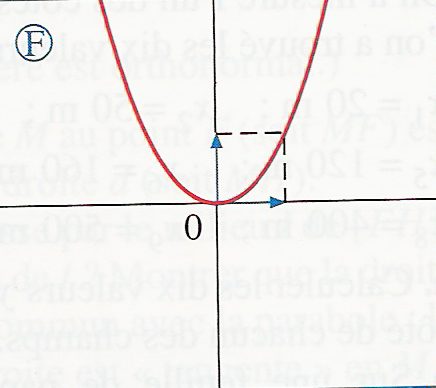
\includegraphics[width=5cm]{images/F.png} \qquad \quad \quad
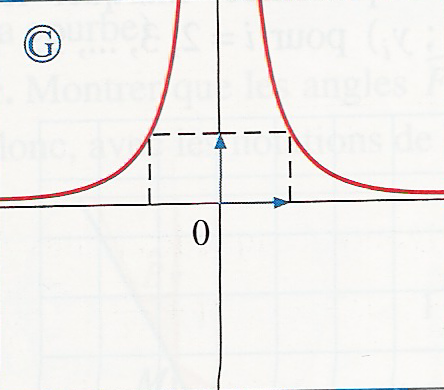
\includegraphics[width=5cm]{images/G.png}

\bigskip

\bigskip

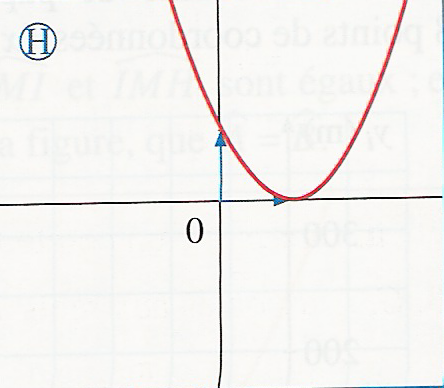
\includegraphics[width=5cm]{images/H.png} \qquad \qquad \quad
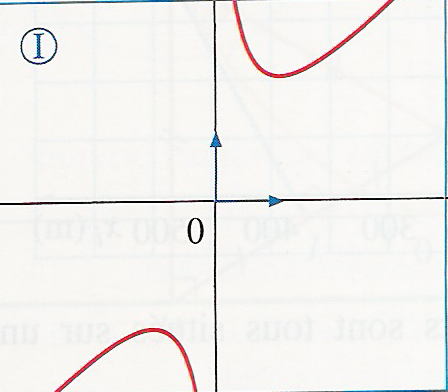
\includegraphics[width=5cm]{images/I.png} \qquad \qquad \quad
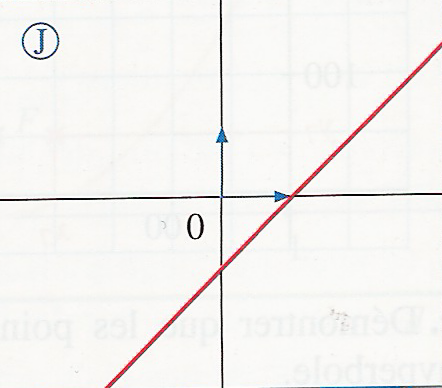
\includegraphics[width=5cm]{images/J.png} 


\end{document}
